\documentclass[a4paper]{article}

% subfile handling packages
\usepackage{subfiles}
\newcommand{\onlyinsubfile}[1]{#1}
\newcommand{\notinsubfile}[1]{}

% document packages
\usepackage[top=1in, bottom=1.25in, left=1.25in, right=1.25in]{geometry}
\usepackage{amsmath}
\usepackage{multicol}
\usepackage{caption}
\usepackage{subcaption}
\usepackage{graphicx}
\usepackage{multirow}
\usepackage{tabulary}
\usepackage{hhline}
\usepackage{indentfirst}
\RequirePackage{ltxcmds}[2010/12/07]
\graphicspath{{../../images/}}
%\graphicspath
\usepackage{float}
\usepackage{amsfonts}
\usepackage{hyperref}
\usepackage{footnote}
\makesavenoteenv{tabular}
%opening
\title{Shot noise study}
\author{}
\date{}


\begin{document}
\maketitle

\section{Introduction}\label{sec:intro}

This document describes a model to simulate the experimental results of the characterization of two homodyne receivers.
\par
The average current output for a homodyne receiver, with coherent input signals $S_1=\sqrt{P_1}e^{i\theta}$ and $S_2=\sqrt{P_2}e^{i\epsilon}$, is given by:
\begin{equation}
I=\eta\sqrt{P_1P_2}\cos\Delta\phi,
\end{equation}
where $\Delta\phi=\theta-\epsilon$ is the phase difference between the two input signals. The current variance introduced by the statistical nature of the photon-number, shot noise, is given by:
\begin{equation}
(\Delta I)^2=\eta(P_1+P_2).
\end{equation}
If only one signal input is used (for example $P_1\neq0\wedge P_2=0$), the output will be purely noise and it's amplitude should scale linearly with the signal power. In addition to the shot noise contribution, two other noise sources are commonly present: 
\begin{itemize}
\item thermal noise, originating from the detector’s electronics and which is independent from the power of the applied signal;
\item relative intensity noise, originating from instabilities in the power level of the used laser.
\end{itemize}
The first of these is independent of the laser power while the latter scales with its square.

\section{Functional Description}

A simplified diagram of the system being simulated is presented in Figures~\ref{fig:singleH}. One of the Local Oscillator block is set to a zero amplitude output (0~W), while the other's power is set at different values to allow for a study of the dynamic properties of the system. The two signals are mixed with a Balanced Beam Splitter and are subsequently evaluated with recourse to a Homodyne Receiver.
\par
Both thermal and shot noise were considered for this simulation, the thermal noise amplitude was set to coincide with the value observed in the experimental results.

\begin{figure}[h]
\centering
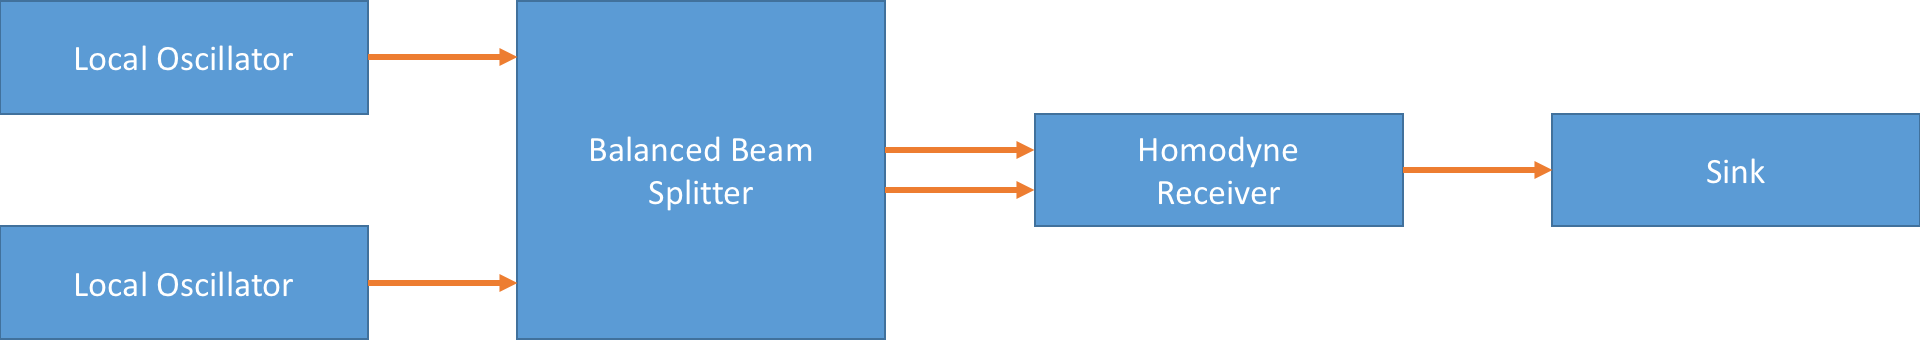
\includegraphics[width=\linewidth]{singlehomodyneSimuBlock.png}
\caption{Overview of the optical system being simulated.}
\label{fig:singleH}
\end{figure}

\begin{table}[H]
\centering
\begin{tabular}{c|c}
System Blocks          & netxpto Blocks       \\ \hline
Local Oscillator       & LocalOscillator      \\
Homodyne Receiver      & I\_HomodyneReceiver   \\
Balanced Beam Splitter & BalancedBeamSplitter
\end{tabular}
\end{table}

\section{Required files}\label{Required files}

Header Files
\begin{table}[H]
\centering
\begin{tabulary}{1.0\textwidth}{|L|L|}
\hline
\textbf{File}              & \textbf{Description} 				            \\ \hline
netxpto.h                  & Generic purpose simulator definitions.	        \\ \hline
local\_oscillator.h        & Generates continuous coherent signal.            \\ \hline
balanced\_beam\_splitter.h & Mixes the two input signals into two outputs.    \\ \hline
homodyne\_reciever.h       & Performs coherent detection on the input signal. \\ \hline
sink.h                     & Closes any unused signals.                       \\ \hline
\end{tabulary}
\end{table}
%
Source Files
\begin{table}[H]
\centering
\begin{tabulary}{1.0\textwidth}{|L|L|}
\hline
\textbf{File}                & \textbf{Description} 					          \\ \hline
netxpto.cpp                  & Generic purpose simulator definitions.	          \\ \hline
local\_oscillator.cpp        & Generates continuous coherent signal.            \\ \hline
balanced\_beam\_splitter.cpp & Mixes the two input signals into two outputs.    \\ \hline
homodyne\_reciever.cpp       & Performs coherent detection on the input signal. \\ \hline
sink.cpp                     & Closes any unused signals.                       \\ \hline
\end{tabulary}
\end{table}


\section{System Input Parameters}

This system takes into account the following input parameters:
\begin{table}[H]
\centering
\begin{tabulary}{1.0\textwidth}{|C|C|}
\hline
\textbf{System Parameters} & \textbf{Description}                                                                   \\ \hline
numberOfBitsGenerated      & Gives the number of bits to be simulated                                               \\ \hline  
bitPeriod                  & Sets the time between adjacent bits                                                    \\ \hline 
samplesPerSymbol           & Establishes the number of samples each bit in the string is given                      \\ \hline
localOscillatorPower\_dBm1 & Sets the optical power, in units of dBm, of the varied amplitude signal                \\ \hline  
localOscillatorPower2      & Sets the optical power, in units of W, of the constant zero amplitude signal           \\ \hline  
localOscillatorPhase1      & Sets the initial phase of the local oscillator used for reference                      \\ \hline 
localOscillatorPhase2      & Sets the initial phase of the local oscillator used for signal                         \\ \hline  
transferMatrix             & Sets the transfer matrix of the beam splitter used in the homodyne detector            \\ \hline  
responsivity               & Sets the responsivity of the photodiodes used in the homodyne detector                 \\ \hline  
amplification              & Sets the amplification of the trans-impedance amplifier used in the homodyne detector  \\ \hline  
electricalNoiseAmplitude   & Sets the amplitude of the gaussian thermal noise added in the homodyne detector        \\ \hline
shotNoise                  & Chooses if quantum shot noise is used in the simulation                                \\ \hline
\end{tabulary}
\end{table}		

\section{Inputs}

This system takes no inputs.

\pagebreak
\section{Outputs}

The system outputs the following objects:
\begin{itemize}
\item Signals:
\begin{itemize}
\item Local Oscillator Optical Reference; (S$_{1}$)
\item Local Oscillator Optical Signal; (S$_{2}$)
\item Beam Splitter Outputs; (S$_{3}$, S$_{4}$)
\item Homodyne Detector Electrical Output; (S$_{5}$)
\end{itemize}
\end{itemize}	

\section{Simulation Results}\label{subsec:SHresults}

The following results show the dependence of the noise variance with the signal power, expressed in the value of the average photon number per pulse. Experimental results of the characterization of two different balanced homodyne detectors, obtained under the same conditions as the ones stipulated for the simulation, are presented in green and purple points alongside their respective quadratic fits. The thermal noise level is presented as a yellow line. The simulation results are presented as red points.

\begin{figure}[h]
\centering
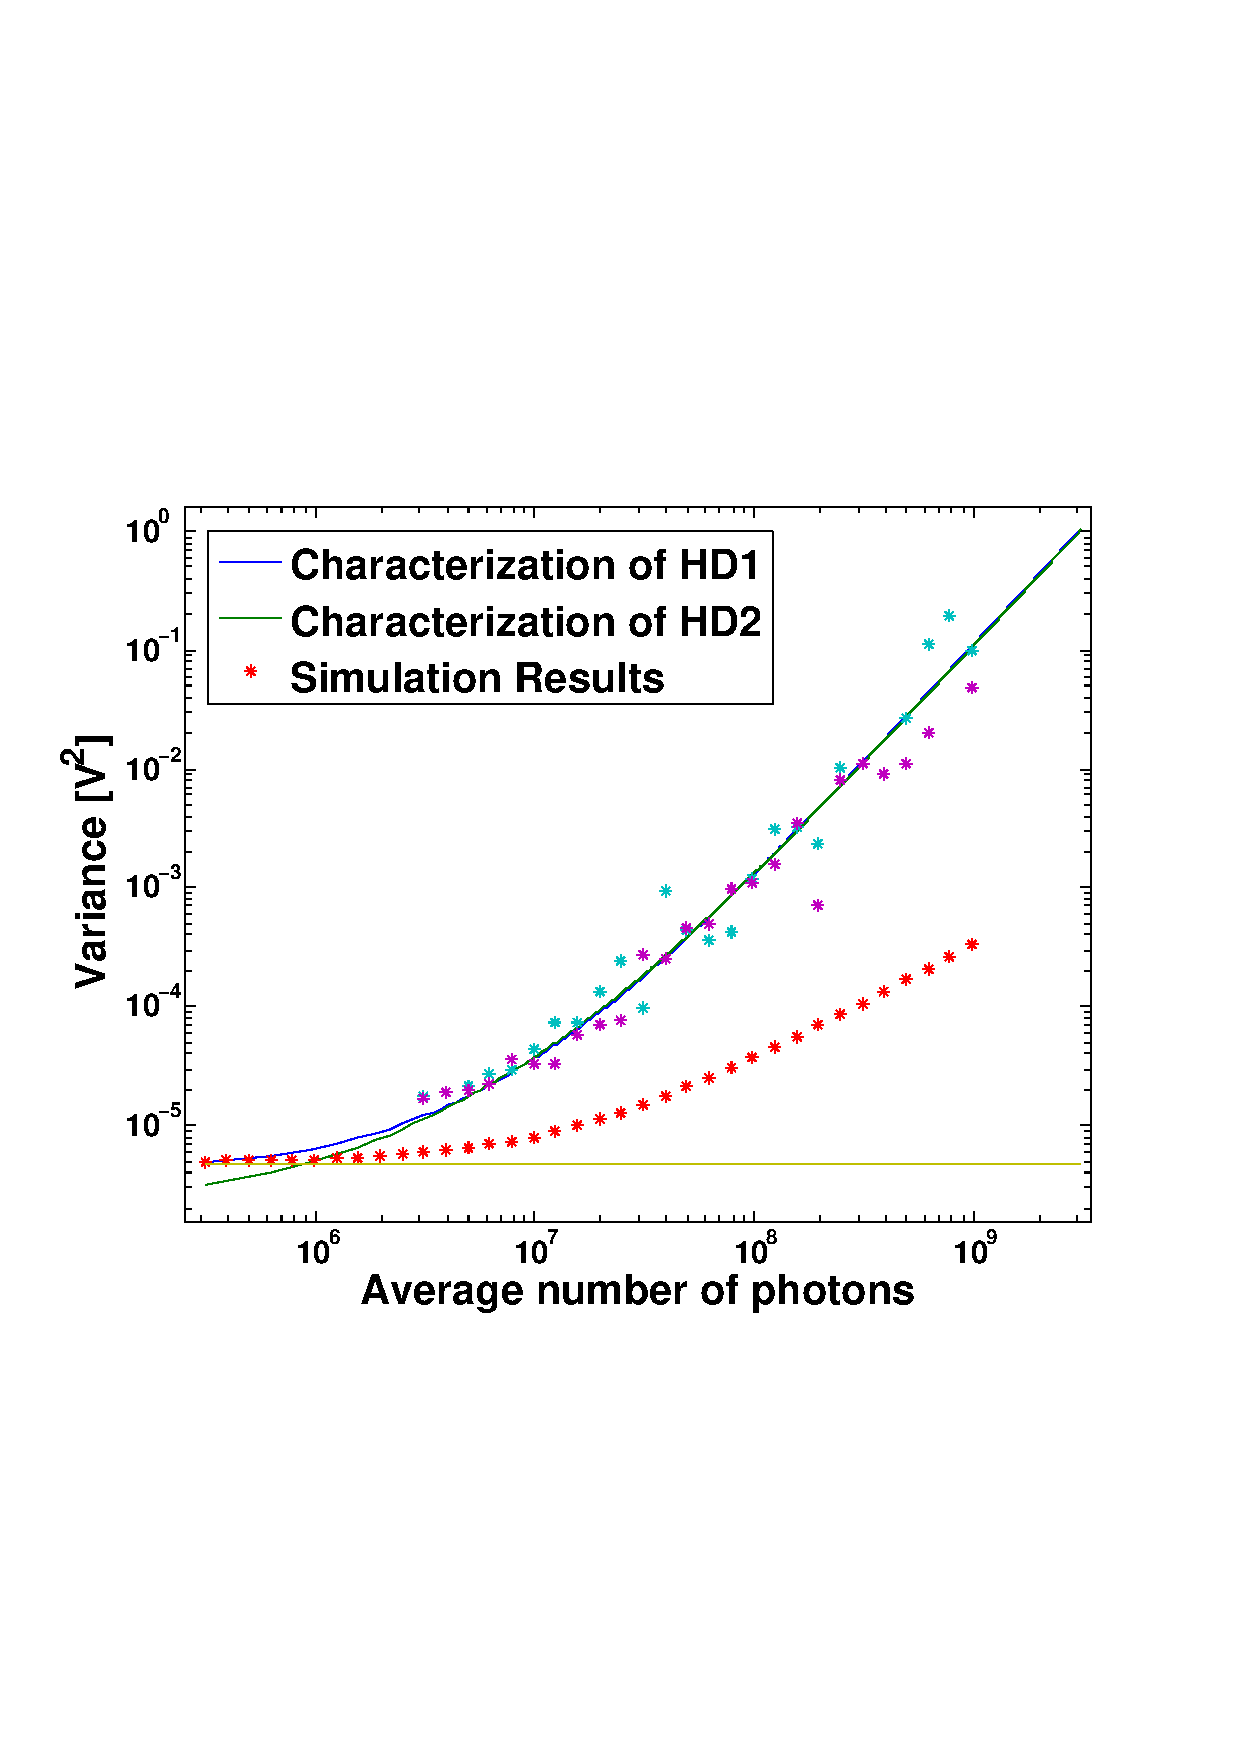
\includegraphics[width=\linewidth, trim= 0mm 60mm 0mm 70mm]{simulationresults1.pdf}
\caption{Noise variance in function of signal power.}
\label{fig:withquad}
\end{figure}

In Figure~\ref{fig:withquad} one can see that all results tend to the same value of thermal noise, however, simulated and experimental results evolve with different rates with signal power, this is mainly due to the existence of noise sources not considered in the simulation, moreover, setting the quadratic parameter in the experimental fit to 0 results yields the results presented in Figure~\ref{fig:withoutquad}, where the difference between the experimental fits and simulated results can be seen to not be as dramatic as before. The simulation and experimental  fits are, respectively:

\begin{table}[H]
\centering
\begin{tabular}{rc}
y=  & p$_0$+p$_1x$            \\
p$_0$= & 4.816$\times10^{-06}$\\
p$_1$= & 3.277$\times10^{-13}$ 
\end{tabular}
\end{table}

\begin{table}[H]
\centering
\begin{tabular}{rc}
y=  & p$_0$+p$_1x$+p$_2x^2$   \\
p$_0$= & 4.164$\times10^{-6}$ \\
p$_1$= & 2.183$\times10^{-12}$\\
p$_2$= & 1.069$\times10^{-19}$                 
\end{tabular}
\end{table}

\begin{table}[H]
\centering
\begin{tabular}{rc}
y=  & p$_0$+p$_1x$+p$_2x^2$   \\
p$_0$= & 2.357$\times10^{-6}$ \\
p$_1$= & 2.527$\times10^{-12}$\\
p$_2$= & 1.038$\times10^{-19}$                 
\end{tabular}
\end{table}

The linear parameters from the experimental fits are one order of magnitude above the linear parameter from the simulation fit, the reasons for this mismatch are still under study.

\begin{figure}[h]
\centering
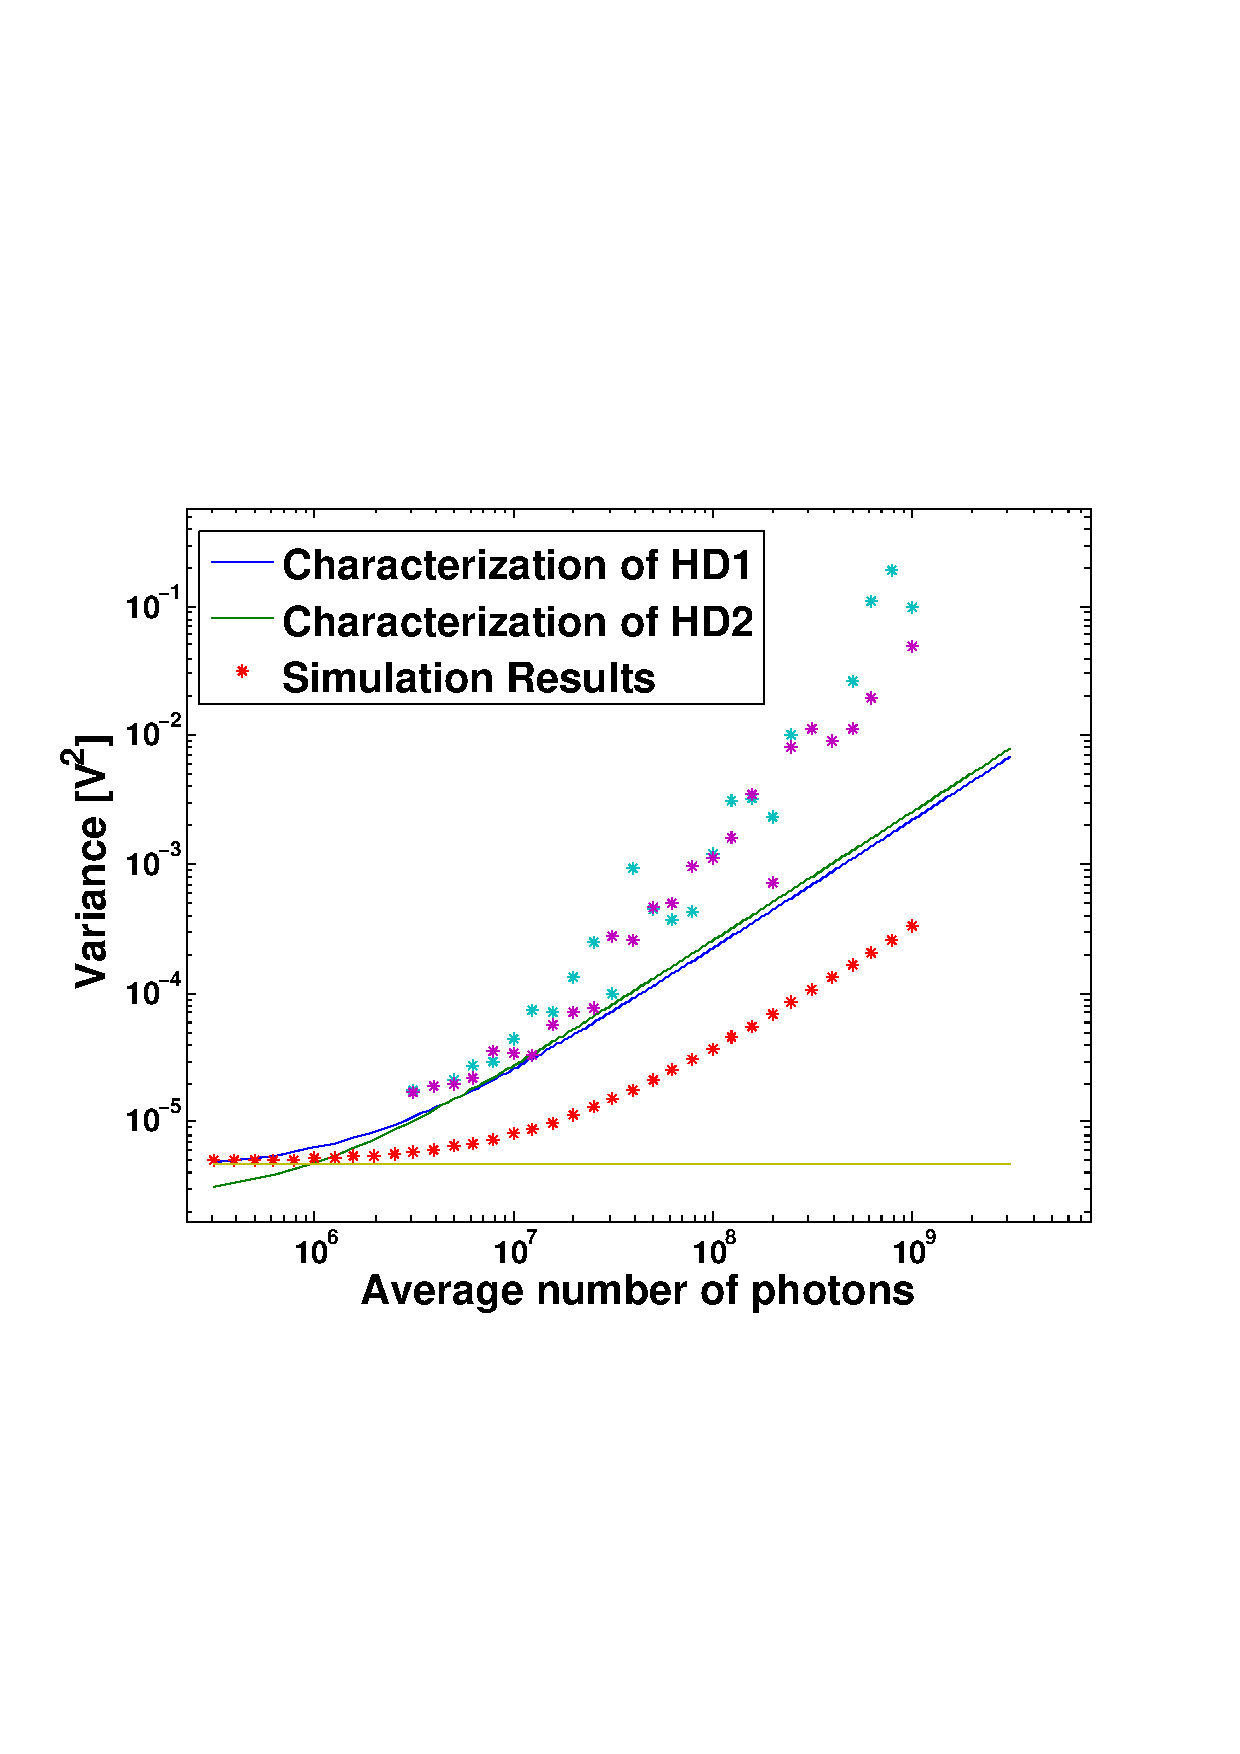
\includegraphics[width=\linewidth, trim= 0mm 60mm 0mm 70mm]{simulationresults2.pdf}
\caption{Noise variance in function of signal power with quadratic parameter deactivated.}
\label{fig:withoutquad}
\end{figure}

\section{Block Description}

\subsection{Homodyne Receiver}
\subfile{../../lib/tex/i_homodyne_reciever}

\subsection{Local Oscillator}
\subfile{../../lib/tex/localoscillator}

\subsection{Beam Splitter}
\subfile{../../lib/tex/beamsplitter}

\subsection{Photodiode}
\subfile{../../lib/tex/photodiode}

\subsection{Amplifier}
\subfile{../../lib/tex/ideal_amplifier}

\subsection{Electrical Filter}
\subfile{../../lib/tex/pulse_shaper}

\section{Known Problems}
\begin{enumerate}
    \item Homodyne Super-Block not functioning
\end{enumerate}


%\bibliographystyle{unsrt}
%\bibliography{bibliography}
\end{document} 